\begin{frame}{The Ehrenfest Urn Model} %intro
    Diffusion of a gas as \alert{stochastic process}
    \begin{itemize}
      \item $N$ particles
      \item 2 boxes
      \item discretized time steps
    \end{itemize}
   
    \begin{figure}
      \begin{center}
        





\tikzset{every picture/.style={line width=0.75pt}} %set default line width to 0.75pt        

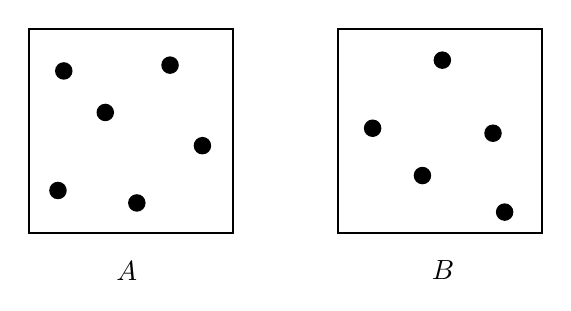
\begin{tikzpicture}[x=0.75pt,y=0.75pt,yscale=-1,xscale=1]
%uncomment if require: \path (0,375); %set diagram left start at 0, and has height of 375

%Shape: Square [id:dp5886506825268709] 
\draw   (181,91.16) -- (279.34,91.16) -- (279.34,189.5) -- (181,189.5) -- cycle ;
%Shape: Square [id:dp24242986167867575] 
\draw   (330,91.16) -- (428.34,91.16) -- (428.34,189.5) -- (330,189.5) -- cycle ;
%Shape: Circle [id:dp48354636802020234] 
\draw  [fill={rgb, 255:red, 0; green, 0; blue, 0 }  ,fill opacity=1 ] (194.19,111.5) .. controls (194.19,109.46) and (195.85,107.8) .. (197.9,107.8) .. controls (199.94,107.8) and (201.6,109.46) .. (201.6,111.5) .. controls (201.6,113.55) and (199.94,115.21) .. (197.9,115.21) .. controls (195.85,115.21) and (194.19,113.55) .. (194.19,111.5) -- cycle ;
%Shape: Circle [id:dp8547166774432848] 
\draw  [fill={rgb, 255:red, 0; green, 0; blue, 0 }  ,fill opacity=1 ] (214.19,131.5) .. controls (214.19,129.46) and (215.85,127.8) .. (217.9,127.8) .. controls (219.94,127.8) and (221.6,129.46) .. (221.6,131.5) .. controls (221.6,133.55) and (219.94,135.21) .. (217.9,135.21) .. controls (215.85,135.21) and (214.19,133.55) .. (214.19,131.5) -- cycle ;
%Shape: Circle [id:dp3635316819967491] 
\draw  [fill={rgb, 255:red, 0; green, 0; blue, 0 }  ,fill opacity=1 ] (191.39,169.1) .. controls (191.39,167.06) and (193.05,165.4) .. (195.1,165.4) .. controls (197.14,165.4) and (198.8,167.06) .. (198.8,169.1) .. controls (198.8,171.15) and (197.14,172.81) .. (195.1,172.81) .. controls (193.05,172.81) and (191.39,171.15) .. (191.39,169.1) -- cycle ;
%Shape: Circle [id:dp504377272845598] 
\draw  [fill={rgb, 255:red, 0; green, 0; blue, 0 }  ,fill opacity=1 ] (245.39,108.7) .. controls (245.39,106.66) and (247.05,105) .. (249.1,105) .. controls (251.14,105) and (252.8,106.66) .. (252.8,108.7) .. controls (252.8,110.75) and (251.14,112.41) .. (249.1,112.41) .. controls (247.05,112.41) and (245.39,110.75) .. (245.39,108.7) -- cycle ;
%Shape: Circle [id:dp40762374287455616] 
\draw  [fill={rgb, 255:red, 0; green, 0; blue, 0 }  ,fill opacity=1 ] (229.39,175.1) .. controls (229.39,173.06) and (231.05,171.4) .. (233.1,171.4) .. controls (235.14,171.4) and (236.8,173.06) .. (236.8,175.1) .. controls (236.8,177.15) and (235.14,178.81) .. (233.1,178.81) .. controls (231.05,178.81) and (229.39,177.15) .. (229.39,175.1) -- cycle ;
%Shape: Circle [id:dp8577561818936912] 
\draw  [fill={rgb, 255:red, 0; green, 0; blue, 0 }  ,fill opacity=1 ] (260.99,147.5) .. controls (260.99,145.46) and (262.65,143.8) .. (264.7,143.8) .. controls (266.74,143.8) and (268.4,145.46) .. (268.4,147.5) .. controls (268.4,149.55) and (266.74,151.21) .. (264.7,151.21) .. controls (262.65,151.21) and (260.99,149.55) .. (260.99,147.5) -- cycle ;
%Shape: Circle [id:dp3598710056160941] 
\draw  [fill={rgb, 255:red, 0; green, 0; blue, 0 }  ,fill opacity=1 ] (376.59,106.3) .. controls (376.59,104.26) and (378.25,102.6) .. (380.3,102.6) .. controls (382.34,102.6) and (384,104.26) .. (384,106.3) .. controls (384,108.35) and (382.34,110.01) .. (380.3,110.01) .. controls (378.25,110.01) and (376.59,108.35) .. (376.59,106.3) -- cycle ;
%Shape: Circle [id:dp8070234513651793] 
\draw  [fill={rgb, 255:red, 0; green, 0; blue, 0 }  ,fill opacity=1 ] (342.99,139.1) .. controls (342.99,137.06) and (344.65,135.4) .. (346.7,135.4) .. controls (348.74,135.4) and (350.4,137.06) .. (350.4,139.1) .. controls (350.4,141.15) and (348.74,142.81) .. (346.7,142.81) .. controls (344.65,142.81) and (342.99,141.15) .. (342.99,139.1) -- cycle ;
%Shape: Circle [id:dp3126762302018198] 
\draw  [fill={rgb, 255:red, 0; green, 0; blue, 0 }  ,fill opacity=1 ] (366.99,161.9) .. controls (366.99,159.86) and (368.65,158.2) .. (370.7,158.2) .. controls (372.74,158.2) and (374.4,159.86) .. (374.4,161.9) .. controls (374.4,163.95) and (372.74,165.61) .. (370.7,165.61) .. controls (368.65,165.61) and (366.99,163.95) .. (366.99,161.9) -- cycle ;
%Shape: Circle [id:dp24135298904714841] 
\draw  [fill={rgb, 255:red, 0; green, 0; blue, 0 }  ,fill opacity=1 ] (406.59,179.5) .. controls (406.59,177.46) and (408.25,175.8) .. (410.3,175.8) .. controls (412.34,175.8) and (414,177.46) .. (414,179.5) .. controls (414,181.55) and (412.34,183.21) .. (410.3,183.21) .. controls (408.25,183.21) and (406.59,181.55) .. (406.59,179.5) -- cycle ;
%Shape: Circle [id:dp9432634536780442] 
\draw  [fill={rgb, 255:red, 0; green, 0; blue, 0 }  ,fill opacity=1 ] (400.99,141.5) .. controls (400.99,139.46) and (402.65,137.8) .. (404.7,137.8) .. controls (406.74,137.8) and (408.4,139.46) .. (408.4,141.5) .. controls (408.4,143.55) and (406.74,145.21) .. (404.7,145.21) .. controls (402.65,145.21) and (400.99,143.55) .. (400.99,141.5) -- cycle ;

% Text Node
\draw (221.73,201.87) node [anchor=north west][inner sep=0.75pt]    {$\text{A}$};
% Text Node
\draw (373.8,201.54) node [anchor=north west][inner sep=0.75pt]    {$\text{B}$};


\end{tikzpicture}
      \end{center}
    \end{figure}

  \end{frame}

  \begin{frame}{The Ehrenfest Urn Model}
    At each time step:
    \begin{itemize}
      \item<1-> \alert<1>{a particle is selected at random among the $N$ possible ones}
      \item<2-> \alert<2>{it is extracted from its box}
      \item<3-> \alert<3>{a box is selected at random}
      \item<4-> \alert<4>{the particle is put in the selected box}
    \end{itemize}

    \medskip
        \begin{figure}[b]
        \begin{center}
            \only<1>{
\tikzset{every picture/.style={line width=0.75pt}} %set default line width to 0.75pt 
    

\begin{tikzpicture}[x=0.75pt,y=0.75pt,yscale=-1,xscale=1]
%uncomment if require: \path (0,375); %set diagram left start at 0, and has height of 375

%Shape: Square [id:dp5886506825268709] 
\draw   (181,91.16) -- (279.34,91.16) -- (279.34,189.5) -- (181,189.5) -- cycle ;
%Shape: Square [id:dp24242986167867575] 
\draw   (330,91.16) -- (428.34,91.16) -- (428.34,189.5) -- (330,189.5) -- cycle ;
%Shape: Circle [id:dp48354636802020234] 
\draw  [fill={rgb, 255:red, 0; green, 0; blue, 0 }  ,fill opacity=1 ] (194.19,111.5) .. controls (194.19,109.46) and (195.85,107.8) .. (197.9,107.8) .. controls (199.94,107.8) and (201.6,109.46) .. (201.6,111.5) .. controls (201.6,113.55) and (199.94,115.21) .. (197.9,115.21) .. controls (195.85,115.21) and (194.19,113.55) .. (194.19,111.5) -- cycle ;
%Shape: Circle [id:dp8547166774432848] 
\draw  [fill={rgb, 255:red, 0; green, 0; blue, 0 }  ,fill opacity=1 ] (214.19,131.5) .. controls (214.19,129.46) and (215.85,127.8) .. (217.9,127.8) .. controls (219.94,127.8) and (221.6,129.46) .. (221.6,131.5) .. controls (221.6,133.55) and (219.94,135.21) .. (217.9,135.21) .. controls (215.85,135.21) and (214.19,133.55) .. (214.19,131.5) -- cycle ;
%Shape: Circle [id:dp3635316819967491] 
\draw  [fill={rgb, 255:red, 0; green, 0; blue, 0 }  ,fill opacity=1 ] (191.39,169.1) .. controls (191.39,167.06) and (193.05,165.4) .. (195.1,165.4) .. controls (197.14,165.4) and (198.8,167.06) .. (198.8,169.1) .. controls (198.8,171.15) and (197.14,172.81) .. (195.1,172.81) .. controls (193.05,172.81) and (191.39,171.15) .. (191.39,169.1) -- cycle ;
%Shape: Circle [id:dp504377272845598] 
\draw  [fill={rgb, 255:red, 0; green, 0; blue, 0 }  ,fill opacity=1 ] (245.39,108.7) .. controls (245.39,106.66) and (247.05,105) .. (249.1,105) .. controls (251.14,105) and (252.8,106.66) .. (252.8,108.7) .. controls (252.8,110.75) and (251.14,112.41) .. (249.1,112.41) .. controls (247.05,112.41) and (245.39,110.75) .. (245.39,108.7) -- cycle ;
%Shape: Circle [id:dp40762374287455616] 
\draw  [fill={rgb, 255:red, 0; green, 0; blue, 0 }  ,fill opacity=1 ] (229.39,175.1) .. controls (229.39,173.06) and (231.05,171.4) .. (233.1,171.4) .. controls (235.14,171.4) and (236.8,173.06) .. (236.8,175.1) .. controls (236.8,177.15) and (235.14,178.81) .. (233.1,178.81) .. controls (231.05,178.81) and (229.39,177.15) .. (229.39,175.1) -- cycle ;
%Shape: Circle [id:dp8577561818936912] 
\draw  [fill={rgb, 255:red, 0; green, 0; blue, 0 }  ,fill opacity=1 ] (260.99,147.5) .. controls (260.99,145.46) and (262.65,143.8) .. (264.7,143.8) .. controls (266.74,143.8) and (268.4,145.46) .. (268.4,147.5) .. controls (268.4,149.55) and (266.74,151.21) .. (264.7,151.21) .. controls (262.65,151.21) and (260.99,149.55) .. (260.99,147.5) -- cycle ;
%Shape: Circle [id:dp3598710056160941] 
\draw  [color=carminepink  ,draw opacity=1 ][fill=carminepink  ,fill opacity=1 ] (376.59,106.3) .. controls (376.59,104.26) and (378.25,102.6) .. (380.3,102.6) .. controls (382.34,102.6) and (384,104.26) .. (384,106.3) .. controls (384,108.35) and (382.34,110.01) .. (380.3,110.01) .. controls (378.25,110.01) and (376.59,108.35) .. (376.59,106.3) -- cycle ;
%Shape: Circle [id:dp8070234513651793] 
\draw  [fill={rgb, 255:red, 0; green, 0; blue, 0 }  ,fill opacity=1 ] (342.99,139.1) .. controls (342.99,137.06) and (344.65,135.4) .. (346.7,135.4) .. controls (348.74,135.4) and (350.4,137.06) .. (350.4,139.1) .. controls (350.4,141.15) and (348.74,142.81) .. (346.7,142.81) .. controls (344.65,142.81) and (342.99,141.15) .. (342.99,139.1) -- cycle ;
%Shape: Circle [id:dp3126762302018198] 
\draw  [fill={rgb, 255:red, 0; green, 0; blue, 0 }  ,fill opacity=1 ] (366.99,161.9) .. controls (366.99,159.86) and (368.65,158.2) .. (370.7,158.2) .. controls (372.74,158.2) and (374.4,159.86) .. (374.4,161.9) .. controls (374.4,163.95) and (372.74,165.61) .. (370.7,165.61) .. controls (368.65,165.61) and (366.99,163.95) .. (366.99,161.9) -- cycle ;
%Shape: Circle [id:dp24135298904714841] 
\draw  [fill={rgb, 255:red, 0; green, 0; blue, 0 }  ,fill opacity=1 ] (406.59,179.5) .. controls (406.59,177.46) and (408.25,175.8) .. (410.3,175.8) .. controls (412.34,175.8) and (414,177.46) .. (414,179.5) .. controls (414,181.55) and (412.34,183.21) .. (410.3,183.21) .. controls (408.25,183.21) and (406.59,181.55) .. (406.59,179.5) -- cycle ;
%Shape: Circle [id:dp9432634536780442] 
\draw  [fill={rgb, 255:red, 0; green, 0; blue, 0 }  ,fill opacity=1 ] (400.99,141.5) .. controls (400.99,139.46) and (402.65,137.8) .. (404.7,137.8) .. controls (406.74,137.8) and (408.4,139.46) .. (408.4,141.5) .. controls (408.4,143.55) and (406.74,145.21) .. (404.7,145.21) .. controls (402.65,145.21) and (400.99,143.55) .. (400.99,141.5) -- cycle ;

% Text Node
\draw (221.73,201.87) node [anchor=north west][inner sep=0.75pt]    {$\text{A}$};
% Text Node
\draw (373.8,201.54) node [anchor=north west][inner sep=0.75pt]    {$\text{B}$};


\end{tikzpicture}
}
            \only<2>{


\tikzset{every picture/.style={line width=0.75pt}} %set default line width to 0.75pt        

\begin{tikzpicture}[x=0.75pt,y=0.75pt,yscale=-1,xscale=1]
%uncomment if require: \path (0,375); %set diagram left start at 0, and has height of 375

%Shape: Square [id:dp5886506825268709] 
\draw   (181,91.16) -- (279.34,91.16) -- (279.34,189.5) -- (181,189.5) -- cycle ;
%Shape: Square [id:dp24242986167867575] 
\draw   (330,91.16) -- (428.34,91.16) -- (428.34,189.5) -- (330,189.5) -- cycle ;
%Shape: Circle [id:dp48354636802020234] 
\draw  [fill={rgb, 255:red, 0; green, 0; blue, 0 }  ,fill opacity=1 ] (194.19,111.5) .. controls (194.19,109.46) and (195.85,107.8) .. (197.9,107.8) .. controls (199.94,107.8) and (201.6,109.46) .. (201.6,111.5) .. controls (201.6,113.55) and (199.94,115.21) .. (197.9,115.21) .. controls (195.85,115.21) and (194.19,113.55) .. (194.19,111.5) -- cycle ;
%Shape: Circle [id:dp8547166774432848] 
\draw  [fill={rgb, 255:red, 0; green, 0; blue, 0 }  ,fill opacity=1 ] (214.19,131.5) .. controls (214.19,129.46) and (215.85,127.8) .. (217.9,127.8) .. controls (219.94,127.8) and (221.6,129.46) .. (221.6,131.5) .. controls (221.6,133.55) and (219.94,135.21) .. (217.9,135.21) .. controls (215.85,135.21) and (214.19,133.55) .. (214.19,131.5) -- cycle ;
%Shape: Circle [id:dp3635316819967491] 
\draw  [fill={rgb, 255:red, 0; green, 0; blue, 0 }  ,fill opacity=1 ] (191.39,169.1) .. controls (191.39,167.06) and (193.05,165.4) .. (195.1,165.4) .. controls (197.14,165.4) and (198.8,167.06) .. (198.8,169.1) .. controls (198.8,171.15) and (197.14,172.81) .. (195.1,172.81) .. controls (193.05,172.81) and (191.39,171.15) .. (191.39,169.1) -- cycle ;
%Shape: Circle [id:dp504377272845598] 
\draw  [fill={rgb, 255:red, 0; green, 0; blue, 0 }  ,fill opacity=1 ] (245.39,108.7) .. controls (245.39,106.66) and (247.05,105) .. (249.1,105) .. controls (251.14,105) and (252.8,106.66) .. (252.8,108.7) .. controls (252.8,110.75) and (251.14,112.41) .. (249.1,112.41) .. controls (247.05,112.41) and (245.39,110.75) .. (245.39,108.7) -- cycle ;
%Shape: Circle [id:dp40762374287455616] 
\draw  [fill={rgb, 255:red, 0; green, 0; blue, 0 }  ,fill opacity=1 ] (229.39,175.1) .. controls (229.39,173.06) and (231.05,171.4) .. (233.1,171.4) .. controls (235.14,171.4) and (236.8,173.06) .. (236.8,175.1) .. controls (236.8,177.15) and (235.14,178.81) .. (233.1,178.81) .. controls (231.05,178.81) and (229.39,177.15) .. (229.39,175.1) -- cycle ;
%Shape: Circle [id:dp8577561818936912] 
\draw  [fill={rgb, 255:red, 0; green, 0; blue, 0 }  ,fill opacity=1 ] (260.99,147.5) .. controls (260.99,145.46) and (262.65,143.8) .. (264.7,143.8) .. controls (266.74,143.8) and (268.4,145.46) .. (268.4,147.5) .. controls (268.4,149.55) and (266.74,151.21) .. (264.7,151.21) .. controls (262.65,151.21) and (260.99,149.55) .. (260.99,147.5) -- cycle ;
%Shape: Circle [id:dp3598710056160941] 
\draw  [color=carminepink  ,draw opacity=1 ][fill=carminepink  ,fill opacity=1 ] (302.19,225.9) .. controls (302.19,223.86) and (303.85,222.2) .. (305.9,222.2) .. controls (307.94,222.2) and (309.6,223.86) .. (309.6,225.9) .. controls (309.6,227.95) and (307.94,229.61) .. (305.9,229.61) .. controls (303.85,229.61) and (302.19,227.95) .. (302.19,225.9) -- cycle ;
%Shape: Circle [id:dp8070234513651793] 
\draw  [fill={rgb, 255:red, 0; green, 0; blue, 0 }  ,fill opacity=1 ] (342.99,139.1) .. controls (342.99,137.06) and (344.65,135.4) .. (346.7,135.4) .. controls (348.74,135.4) and (350.4,137.06) .. (350.4,139.1) .. controls (350.4,141.15) and (348.74,142.81) .. (346.7,142.81) .. controls (344.65,142.81) and (342.99,141.15) .. (342.99,139.1) -- cycle ;
%Shape: Circle [id:dp3126762302018198] 
\draw  [fill={rgb, 255:red, 0; green, 0; blue, 0 }  ,fill opacity=1 ] (366.99,161.9) .. controls (366.99,159.86) and (368.65,158.2) .. (370.7,158.2) .. controls (372.74,158.2) and (374.4,159.86) .. (374.4,161.9) .. controls (374.4,163.95) and (372.74,165.61) .. (370.7,165.61) .. controls (368.65,165.61) and (366.99,163.95) .. (366.99,161.9) -- cycle ;
%Shape: Circle [id:dp24135298904714841] 
\draw  [fill={rgb, 255:red, 0; green, 0; blue, 0 }  ,fill opacity=1 ] (406.59,179.5) .. controls (406.59,177.46) and (408.25,175.8) .. (410.3,175.8) .. controls (412.34,175.8) and (414,177.46) .. (414,179.5) .. controls (414,181.55) and (412.34,183.21) .. (410.3,183.21) .. controls (408.25,183.21) and (406.59,181.55) .. (406.59,179.5) -- cycle ;
%Shape: Circle [id:dp9432634536780442] 
\draw  [fill={rgb, 255:red, 0; green, 0; blue, 0 }  ,fill opacity=1 ] (400.99,141.5) .. controls (400.99,139.46) and (402.65,137.8) .. (404.7,137.8) .. controls (406.74,137.8) and (408.4,139.46) .. (408.4,141.5) .. controls (408.4,143.55) and (406.74,145.21) .. (404.7,145.21) .. controls (402.65,145.21) and (400.99,143.55) .. (400.99,141.5) -- cycle ;

% Text Node
\draw (221.73,201.87) node [anchor=north west][inner sep=0.75pt]    {$\text{A}$};
% Text Node
\draw (373.8,201.54) node [anchor=north west][inner sep=0.75pt]    {$\text{B}$};


\end{tikzpicture}}
            \only<3>{


\tikzset{every picture/.style={line width=0.75pt}} %set default line width to 0.75pt        

\begin{tikzpicture}[x=0.75pt,y=0.75pt,yscale=-1,xscale=1]
%uncomment if require: \path (0,375); %set diagram left start at 0, and has height of 375

%Shape: Square [id:dp5886506825268709] 
\draw  [color=carminepink  ,draw opacity=1 ] (181,91.16) -- (279.34,91.16) -- (279.34,189.5) -- (181,189.5) -- cycle ;
%Shape: Square [id:dp24242986167867575] 
\draw   (330,91.16) -- (428.34,91.16) -- (428.34,189.5) -- (330,189.5) -- cycle ;
%Shape: Circle [id:dp48354636802020234] 
\draw  [fill={rgb, 255:red, 0; green, 0; blue, 0 }  ,fill opacity=1 ] (194.19,111.5) .. controls (194.19,109.46) and (195.85,107.8) .. (197.9,107.8) .. controls (199.94,107.8) and (201.6,109.46) .. (201.6,111.5) .. controls (201.6,113.55) and (199.94,115.21) .. (197.9,115.21) .. controls (195.85,115.21) and (194.19,113.55) .. (194.19,111.5) -- cycle ;
%Shape: Circle [id:dp8547166774432848] 
\draw  [fill={rgb, 255:red, 0; green, 0; blue, 0 }  ,fill opacity=1 ] (214.19,131.5) .. controls (214.19,129.46) and (215.85,127.8) .. (217.9,127.8) .. controls (219.94,127.8) and (221.6,129.46) .. (221.6,131.5) .. controls (221.6,133.55) and (219.94,135.21) .. (217.9,135.21) .. controls (215.85,135.21) and (214.19,133.55) .. (214.19,131.5) -- cycle ;
%Shape: Circle [id:dp3635316819967491] 
\draw  [fill={rgb, 255:red, 0; green, 0; blue, 0 }  ,fill opacity=1 ] (191.39,169.1) .. controls (191.39,167.06) and (193.05,165.4) .. (195.1,165.4) .. controls (197.14,165.4) and (198.8,167.06) .. (198.8,169.1) .. controls (198.8,171.15) and (197.14,172.81) .. (195.1,172.81) .. controls (193.05,172.81) and (191.39,171.15) .. (191.39,169.1) -- cycle ;
%Shape: Circle [id:dp504377272845598] 
\draw  [fill={rgb, 255:red, 0; green, 0; blue, 0 }  ,fill opacity=1 ] (245.39,108.7) .. controls (245.39,106.66) and (247.05,105) .. (249.1,105) .. controls (251.14,105) and (252.8,106.66) .. (252.8,108.7) .. controls (252.8,110.75) and (251.14,112.41) .. (249.1,112.41) .. controls (247.05,112.41) and (245.39,110.75) .. (245.39,108.7) -- cycle ;
%Shape: Circle [id:dp40762374287455616] 
\draw  [fill={rgb, 255:red, 0; green, 0; blue, 0 }  ,fill opacity=1 ] (229.39,175.1) .. controls (229.39,173.06) and (231.05,171.4) .. (233.1,171.4) .. controls (235.14,171.4) and (236.8,173.06) .. (236.8,175.1) .. controls (236.8,177.15) and (235.14,178.81) .. (233.1,178.81) .. controls (231.05,178.81) and (229.39,177.15) .. (229.39,175.1) -- cycle ;
%Shape: Circle [id:dp8577561818936912] 
\draw  [fill={rgb, 255:red, 0; green, 0; blue, 0 }  ,fill opacity=1 ] (260.99,147.5) .. controls (260.99,145.46) and (262.65,143.8) .. (264.7,143.8) .. controls (266.74,143.8) and (268.4,145.46) .. (268.4,147.5) .. controls (268.4,149.55) and (266.74,151.21) .. (264.7,151.21) .. controls (262.65,151.21) and (260.99,149.55) .. (260.99,147.5) -- cycle ;
%Shape: Circle [id:dp3598710056160941] 
\draw  [color=carminepink  ,draw opacity=1 ][fill={rgb, 255:red, 203; green, 65; blue, 84 }  ,fill opacity=1 ] (302.19,225.9) .. controls (302.19,223.86) and (303.85,222.2) .. (305.9,222.2) .. controls (307.94,222.2) and (309.6,223.86) .. (309.6,225.9) .. controls (309.6,227.95) and (307.94,229.61) .. (305.9,229.61) .. controls (303.85,229.61) and (302.19,227.95) .. (302.19,225.9) -- cycle ;
%Shape: Circle [id:dp8070234513651793] 
\draw  [fill={rgb, 255:red, 0; green, 0; blue, 0 }  ,fill opacity=1 ] (342.99,139.1) .. controls (342.99,137.06) and (344.65,135.4) .. (346.7,135.4) .. controls (348.74,135.4) and (350.4,137.06) .. (350.4,139.1) .. controls (350.4,141.15) and (348.74,142.81) .. (346.7,142.81) .. controls (344.65,142.81) and (342.99,141.15) .. (342.99,139.1) -- cycle ;
%Shape: Circle [id:dp3126762302018198] 
\draw  [fill={rgb, 255:red, 0; green, 0; blue, 0 }  ,fill opacity=1 ] (366.99,161.9) .. controls (366.99,159.86) and (368.65,158.2) .. (370.7,158.2) .. controls (372.74,158.2) and (374.4,159.86) .. (374.4,161.9) .. controls (374.4,163.95) and (372.74,165.61) .. (370.7,165.61) .. controls (368.65,165.61) and (366.99,163.95) .. (366.99,161.9) -- cycle ;
%Shape: Circle [id:dp24135298904714841] 
\draw  [fill={rgb, 255:red, 0; green, 0; blue, 0 }  ,fill opacity=1 ] (406.59,179.5) .. controls (406.59,177.46) and (408.25,175.8) .. (410.3,175.8) .. controls (412.34,175.8) and (414,177.46) .. (414,179.5) .. controls (414,181.55) and (412.34,183.21) .. (410.3,183.21) .. controls (408.25,183.21) and (406.59,181.55) .. (406.59,179.5) -- cycle ;
%Shape: Circle [id:dp9432634536780442] 
\draw  [fill={rgb, 255:red, 0; green, 0; blue, 0 }  ,fill opacity=1 ] (400.99,141.5) .. controls (400.99,139.46) and (402.65,137.8) .. (404.7,137.8) .. controls (406.74,137.8) and (408.4,139.46) .. (408.4,141.5) .. controls (408.4,143.55) and (406.74,145.21) .. (404.7,145.21) .. controls (402.65,145.21) and (400.99,143.55) .. (400.99,141.5) -- cycle ;

% Text Node
\draw (221.73,201.87) node [anchor=north west][inner sep=0.75pt]    {$\text{A}$};
% Text Node
\draw (373.8,201.54) node [anchor=north west][inner sep=0.75pt]    {$\text{B}$};


\end{tikzpicture}}
            \only<4>{


\tikzset{every picture/.style={line width=0.75pt}} %set default line width to 0.75pt    
    

\begin{tikzpicture}[x=0.75pt,y=0.75pt,yscale=-1,xscale=1]
%uncomment if require: \path (0,375); %set diagram left start at 0, and has height of 375

%Shape: Square [id:dp5886506825268709] 
\draw  [color=carminepink  ,draw opacity=1 ] (181,91.16) -- (279.34,91.16) -- (279.34,189.5) -- (181,189.5) -- cycle ;
%Shape: Square [id:dp24242986167867575] 
\draw   (330,91.16) -- (428.34,91.16) -- (428.34,189.5) -- (330,189.5) -- cycle ;
%Shape: Circle [id:dp48354636802020234] 
\draw  [fill={rgb, 255:red, 0; green, 0; blue, 0 }  ,fill opacity=1 ] (194.19,111.5) .. controls (194.19,109.46) and (195.85,107.8) .. (197.9,107.8) .. controls (199.94,107.8) and (201.6,109.46) .. (201.6,111.5) .. controls (201.6,113.55) and (199.94,115.21) .. (197.9,115.21) .. controls (195.85,115.21) and (194.19,113.55) .. (194.19,111.5) -- cycle ;
%Shape: Circle [id:dp8547166774432848] 
\draw  [fill={rgb, 255:red, 0; green, 0; blue, 0 }  ,fill opacity=1 ] (214.19,131.5) .. controls (214.19,129.46) and (215.85,127.8) .. (217.9,127.8) .. controls (219.94,127.8) and (221.6,129.46) .. (221.6,131.5) .. controls (221.6,133.55) and (219.94,135.21) .. (217.9,135.21) .. controls (215.85,135.21) and (214.19,133.55) .. (214.19,131.5) -- cycle ;
%Shape: Circle [id:dp3635316819967491] 
\draw  [fill={rgb, 255:red, 0; green, 0; blue, 0 }  ,fill opacity=1 ] (191.39,169.1) .. controls (191.39,167.06) and (193.05,165.4) .. (195.1,165.4) .. controls (197.14,165.4) and (198.8,167.06) .. (198.8,169.1) .. controls (198.8,171.15) and (197.14,172.81) .. (195.1,172.81) .. controls (193.05,172.81) and (191.39,171.15) .. (191.39,169.1) -- cycle ;
%Shape: Circle [id:dp504377272845598] 
\draw  [fill={rgb, 255:red, 0; green, 0; blue, 0 }  ,fill opacity=1 ] (245.39,108.7) .. controls (245.39,106.66) and (247.05,105) .. (249.1,105) .. controls (251.14,105) and (252.8,106.66) .. (252.8,108.7) .. controls (252.8,110.75) and (251.14,112.41) .. (249.1,112.41) .. controls (247.05,112.41) and (245.39,110.75) .. (245.39,108.7) -- cycle ;
%Shape: Circle [id:dp40762374287455616] 
\draw  [fill={rgb, 255:red, 0; green, 0; blue, 0 }  ,fill opacity=1 ] (229.39,175.1) .. controls (229.39,173.06) and (231.05,171.4) .. (233.1,171.4) .. controls (235.14,171.4) and (236.8,173.06) .. (236.8,175.1) .. controls (236.8,177.15) and (235.14,178.81) .. (233.1,178.81) .. controls (231.05,178.81) and (229.39,177.15) .. (229.39,175.1) -- cycle ;
%Shape: Circle [id:dp8577561818936912] 
\draw  [fill={rgb, 255:red, 0; green, 0; blue, 0 }  ,fill opacity=1 ] (260.99,147.5) .. controls (260.99,145.46) and (262.65,143.8) .. (264.7,143.8) .. controls (266.74,143.8) and (268.4,145.46) .. (268.4,147.5) .. controls (268.4,149.55) and (266.74,151.21) .. (264.7,151.21) .. controls (262.65,151.21) and (260.99,149.55) .. (260.99,147.5) -- cycle ;
%Shape: Circle [id:dp3598710056160941] 
\draw  [color=carminepink  ,draw opacity=1 ][fill=carminepink,fill opacity=1 ] (238.99,149.1) .. controls (238.99,147.06) and (240.65,145.4) .. (242.7,145.4) .. controls (244.74,145.4) and (246.4,147.06) .. (246.4,149.1) .. controls (246.4,151.15) and (244.74,152.81) .. (242.7,152.81) .. controls (240.65,152.81) and (238.99,151.15) .. (238.99,149.1) -- cycle ;
%Shape: Circle [id:dp8070234513651793] 
\draw  [fill={rgb, 255:red, 0; green, 0; blue, 0 }  ,fill opacity=1 ] (342.99,139.1) .. controls (342.99,137.06) and (344.65,135.4) .. (346.7,135.4) .. controls (348.74,135.4) and (350.4,137.06) .. (350.4,139.1) .. controls (350.4,141.15) and (348.74,142.81) .. (346.7,142.81) .. controls (344.65,142.81) and (342.99,141.15) .. (342.99,139.1) -- cycle ;
%Shape: Circle [id:dp3126762302018198] 
\draw  [fill={rgb, 255:red, 0; green, 0; blue, 0 }  ,fill opacity=1 ] (366.99,161.9) .. controls (366.99,159.86) and (368.65,158.2) .. (370.7,158.2) .. controls (372.74,158.2) and (374.4,159.86) .. (374.4,161.9) .. controls (374.4,163.95) and (372.74,165.61) .. (370.7,165.61) .. controls (368.65,165.61) and (366.99,163.95) .. (366.99,161.9) -- cycle ;
%Shape: Circle [id:dp24135298904714841] 
\draw  [fill={rgb, 255:red, 0; green, 0; blue, 0 }  ,fill opacity=1 ] (406.59,179.5) .. controls (406.59,177.46) and (408.25,175.8) .. (410.3,175.8) .. controls (412.34,175.8) and (414,177.46) .. (414,179.5) .. controls (414,181.55) and (412.34,183.21) .. (410.3,183.21) .. controls (408.25,183.21) and (406.59,181.55) .. (406.59,179.5) -- cycle ;
%Shape: Circle [id:dp9432634536780442] 
\draw  [fill={rgb, 255:red, 0; green, 0; blue, 0 }  ,fill opacity=1 ] (400.99,141.5) .. controls (400.99,139.46) and (402.65,137.8) .. (404.7,137.8) .. controls (406.74,137.8) and (408.4,139.46) .. (408.4,141.5) .. controls (408.4,143.55) and (406.74,145.21) .. (404.7,145.21) .. controls (402.65,145.21) and (400.99,143.55) .. (400.99,141.5) -- cycle ;

% Text Node
\draw (221.73,201.87) node [anchor=north west][inner sep=0.75pt]    {$\text{A}$};
% Text Node
\draw (373.8,201.54) node [anchor=north west][inner sep=0.75pt]    {$\text{B}$};


\end{tikzpicture}}
        \end{center}
        \end{figure}
  \end{frame}

